\documentclass{article}
\usepackage[utf8]{inputenc}
\usepackage{listings}
\lstset{
	language=Octave,
	frame=single,
	xleftmargin=.1\textwidth, xrightmargin=.1\textwidth
}
\usepackage{graphicx}
\usepackage{mathtools, nccmath}
\usepackage[T2A]{fontenc}
\usepackage[utf8]{inputenc}
\usepackage[russian]{babel}
\usepackage{amsmath}
\usepackage[left=2cm,right=2cm,top=2cm,bottom=2.1cm,bindingoffset=0cm]{geometry}
\usepackage{amsfonts}

\graphicspath{{/pic}}
\DeclarePairedDelimiter{\nint}\lfloor\rfloor

\title{Некоторые уражнения из учебника}
\author{Кокорин Илья, M3439}
\date{Вариант № 64}

\begin{document}
	\maketitle
	\section{Задача 3.1}
	
	\subsection{Коды Хемминга}
	
	Рассмотрим коды Хемминга с фиксированным r, $n = 2^r - 1, k = 2^r - r - 1, d = 3$
	
	Граница Хемминга имеет вид $M \leq \frac{q^n}{\sum\limits_{i = 0}^t \binom{n}{i} \cdot (q - 1)^i}$, в случае двоичного кода, у которого $M = 2^k, q = 2$, принимает вид $2^k \leq \frac{2^n}{\sum\limits_{i = 0}^t \binom{n}{i} \cdot (2 - 1)^i} \Rightarrow 2^k \leq \frac{2^n}{\sum\limits_{i = 0}^t \binom{n}{i}} \Rightarrow \sum\limits_{i = 0}^t \binom{n}{i} \leq 2^{n - k}$
	
	Так как $d = 3$, то $t = \nint{\frac{3 - 1}{2}} = 1$, код исправляет любые однократные ошибки
	
	Тогда $ \sum\limits_{i = 0}^t \binom{n}{i} = \binom{n}{0} + \binom{n}{1} = 1 + n = 1 + 2^r -1 = 2^r$
	
	$2^{n - k} = 2^{2^r - 1 - (2^r - r - 1)} = 2^{2^r - 1 - 2^r + r + 1} = 2^r$
	
	Тогда $2^{n - k} = \sum\limits_{i = 0}^t \binom{n}{i} $, то есть код Хемминга удовлетворяет границе Хемминга с равенством.
	
	\subsection{Код Голея}
	
	$n = 23, k = 12, d = 7$
	
	$t = \nint{\frac{7 - 1}{3}} = 3$
	
	Граница Хемминга имеет вид $M \leq \frac{q^n}{\sum\limits_{i = 0}^t \binom{n}{i} \cdot (q - 1)^i}$, в случае двоичного кода, у которого $M = 2^k, q = 2$, принимает вид $2^k \leq \frac{2^n}{\sum\limits_{i = 0}^t \binom{n}{i} \cdot (2 - 1)^i} \Rightarrow 2^k \leq \frac{2^n}{\sum\limits_{i = 0}^t \binom{n}{i}} \Rightarrow \sum\limits_{i = 0}^t \binom{n}{i} \leq 2^{n - k}$
	
	$ \sum\limits_{i = 0}^t \binom{n}{i} = \binom{23}{0} + \binom{23}{1} + \binom{23}{2} + \binom{23}{3} = 2048$
	
	$2^{n - k} = 2^{23 - 12} = 2^11 = 2048$
	
	Тогда $ \sum\limits_{i = 0}^t \binom{n}{i} = 2^{n - k}$, то есть Код Голея удовлетворяет границе Хемминга с равенством.
	
	\section{Задача 3.2}
	
	Рассмотрим коды, дуальные к кодах Хемминга. Код Хемминга имеет параметры $n = 2^r - 1, k = 2^r - r - 1, r = r, d = 3$, и имеет порождающую матрицу $G: 2^r - r - 1 \times 2^r - 1$ и проверочную матрицу $H: r \times 2^r - 1$.
	
	Тогда код, дуальный к Кодам Хемминга, имеет порождающую матрицу $G: r \times 2^r - 1$, проверочную матрицу $2^r - r - 1 \times 2^r - 1$, и минимальное расстояние $d = 2^{r - 1}$
	
	\subsection{Граница Хемминга}
	
	Граница Хемминга имеет вид $M \leq \frac{q^n}{\sum\limits_{i = 0}^t \binom{n}{i} \cdot (q - 1)^i}$, в случае двоичного кода, у которого $M = 2^k, q = 2$, принимает вид $2^k \leq \frac{2^n}{\sum\limits_{i = 0}^t \binom{n}{i} \cdot (2 - 1)^i} \Rightarrow 2^k \leq \frac{2^n}{\sum\limits_{i = 0}^t \binom{n}{i}} \Rightarrow \sum\limits_{i = 0}^t \binom{n}{i} \leq 2^{n - k}$
	
	В силу особенностей кода, дуального к кодам Хемминга, граница имеет вид:
	
	$ \sum\limits_{i = 0}^t \binom{2^r - 1}{i} \leq 2^{2^r - 1- r }$
	
	\subsection{Граница Варшамова-Гилберта}
	
	Граница Варшамова-Гилберта имеет вид $q^{n - k} > \sum\limits_{i = 0}^{d - 2} \binom{n - 1}{i} \cdot (q - 1)^i$
	
	Что в нашем случае превращается в $\sum\limits_{i = 0}^{2^{r - 1} - 2} \binom{2^r - 2}{i} < 2^{2^r - 1 - r}$
	
	\subsection{Нахождение границ}
	
	Решать такие неравенства слишком сложно, давайте промоделируем.
	
	Программа для моделирования приложена к заданию.
	
	Итоговый график выглядит следующим образом:
	
	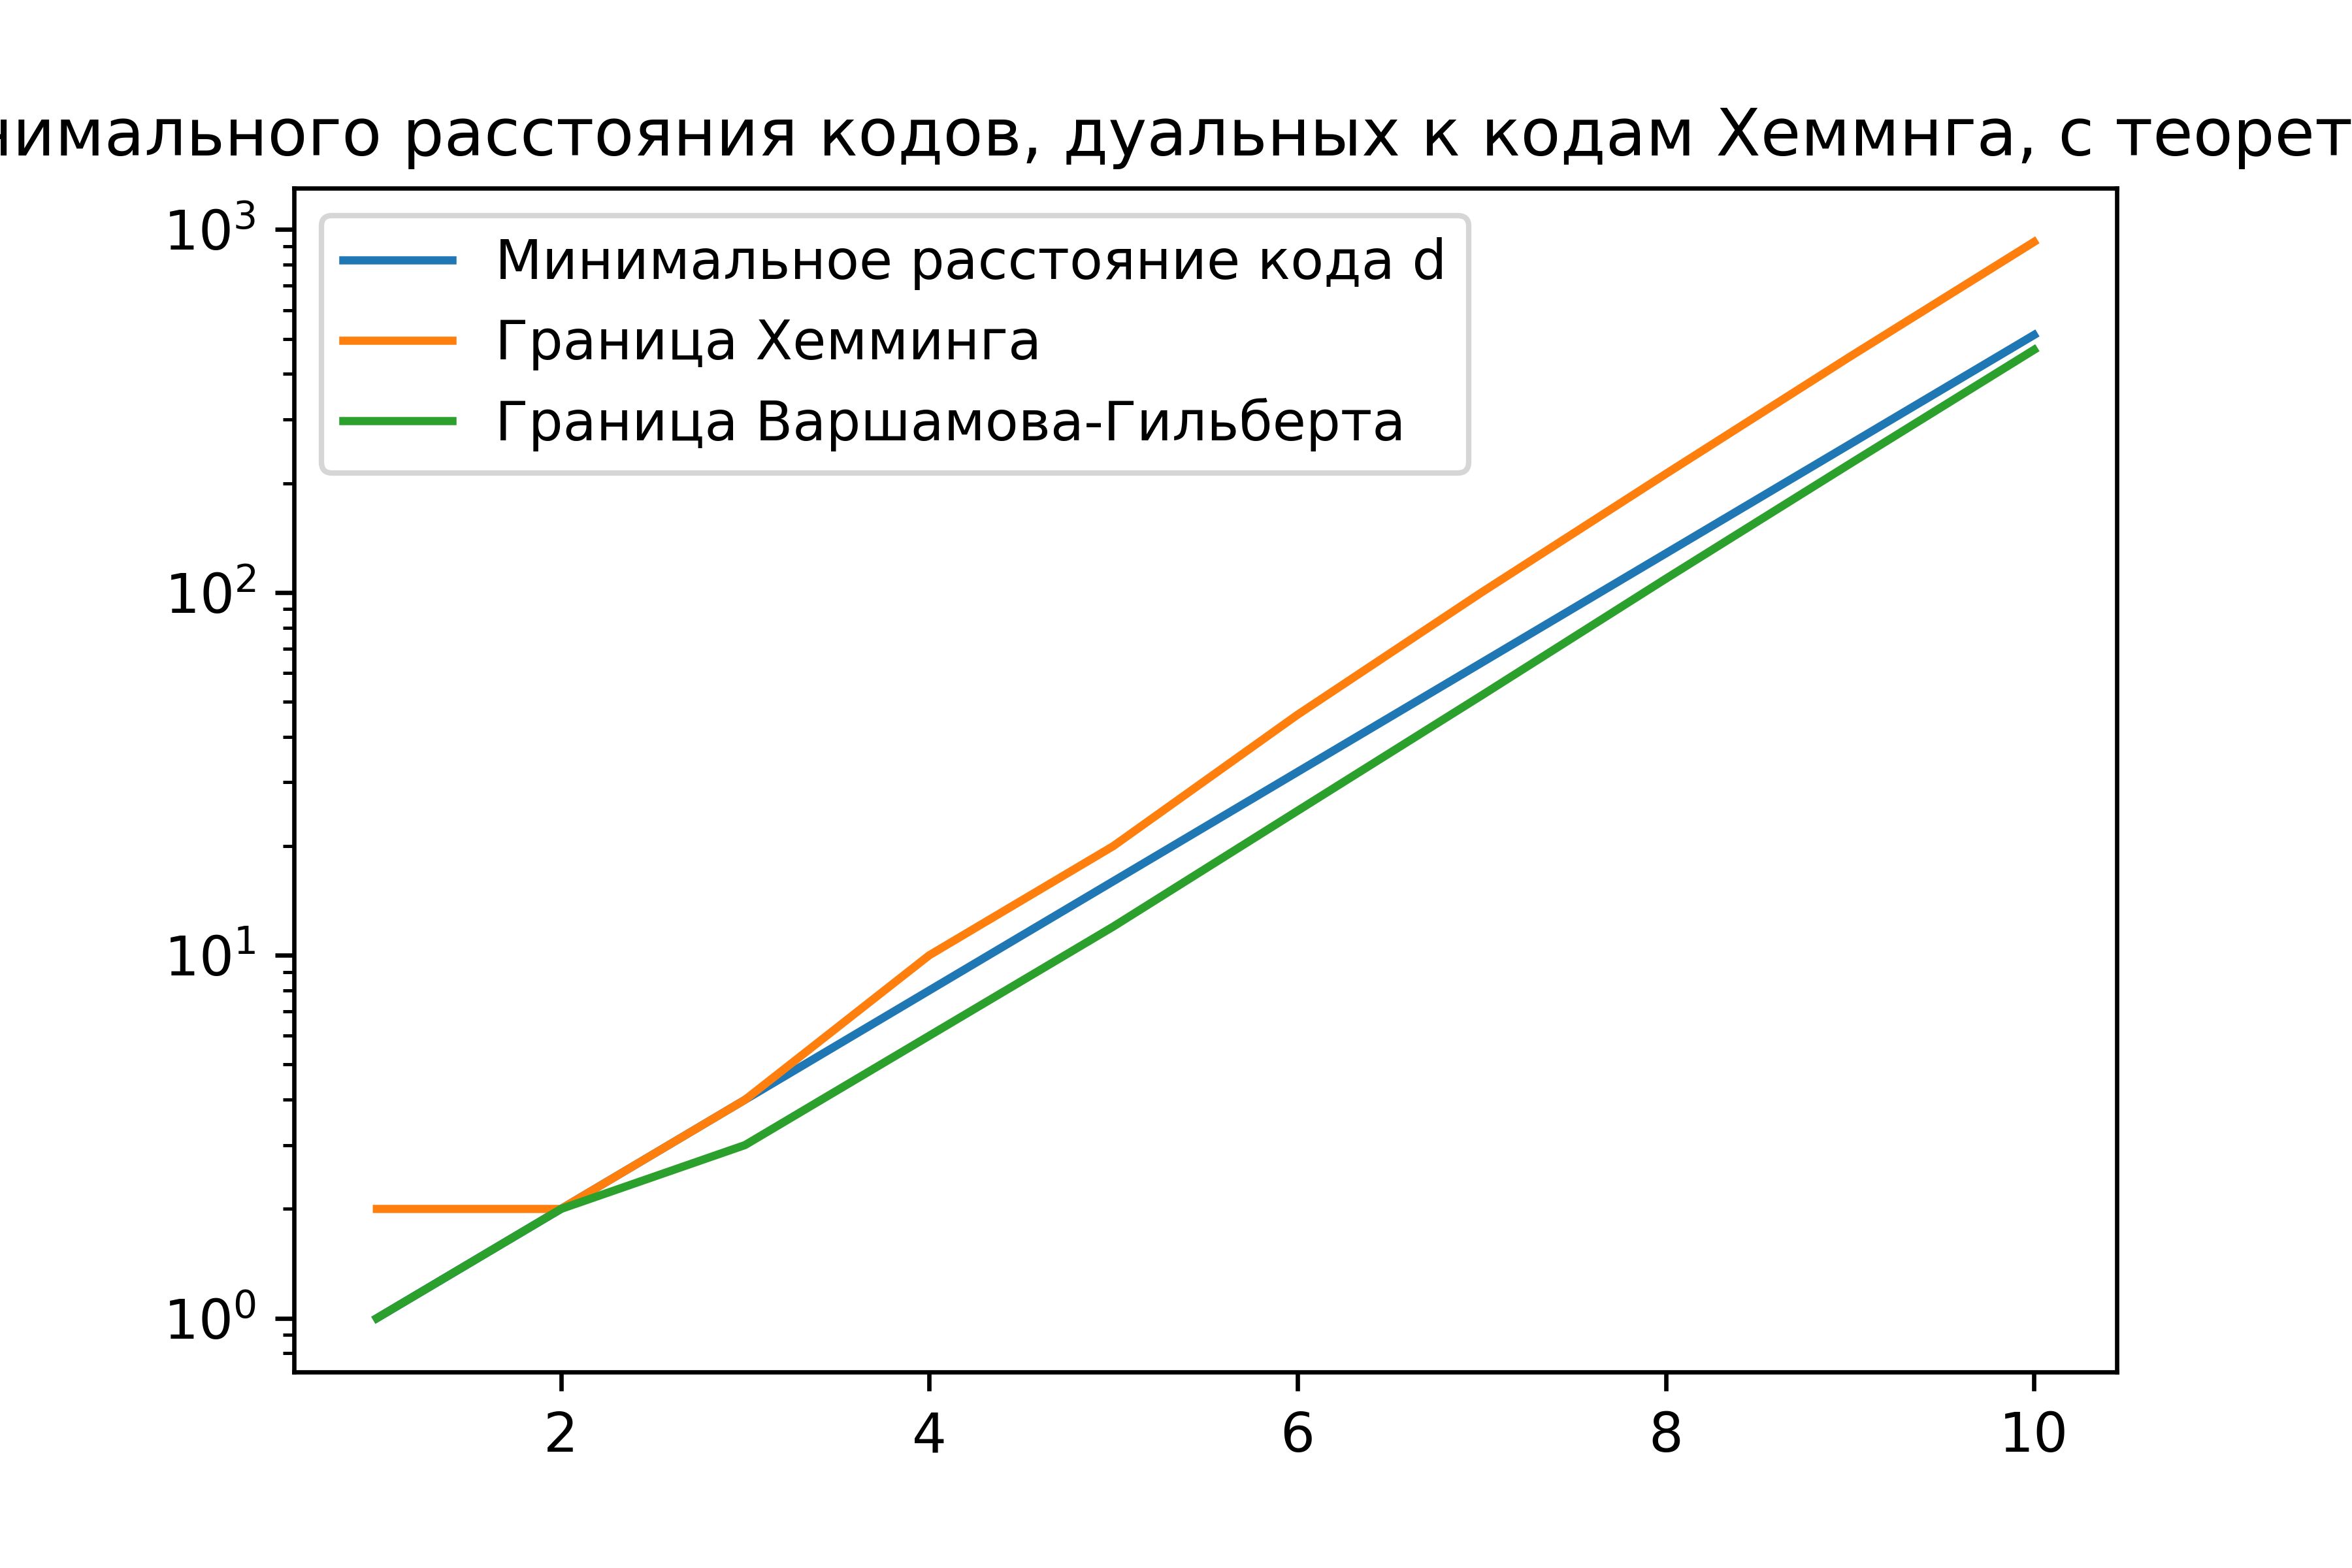
\includegraphics[scale=1]{pic/dist.png}
	
	\section{Задача 3.5}
	
	Рассмотрим коды из таблицы 3.2 с $n \in \{n: 2 \leq n \leq 40\}$
	
	Будем рассматривать только коды с чётными $n$, чтобы получать скорость $R = \frac{1}{2}$
	
	Будем строить для них минимальное расстояние, границу Хемминга и границу Варшамова-Гилберта.
	
	Программа для моделирования приложена к заданию.
	
	Итоговый график выглядит следующим образом:
	
	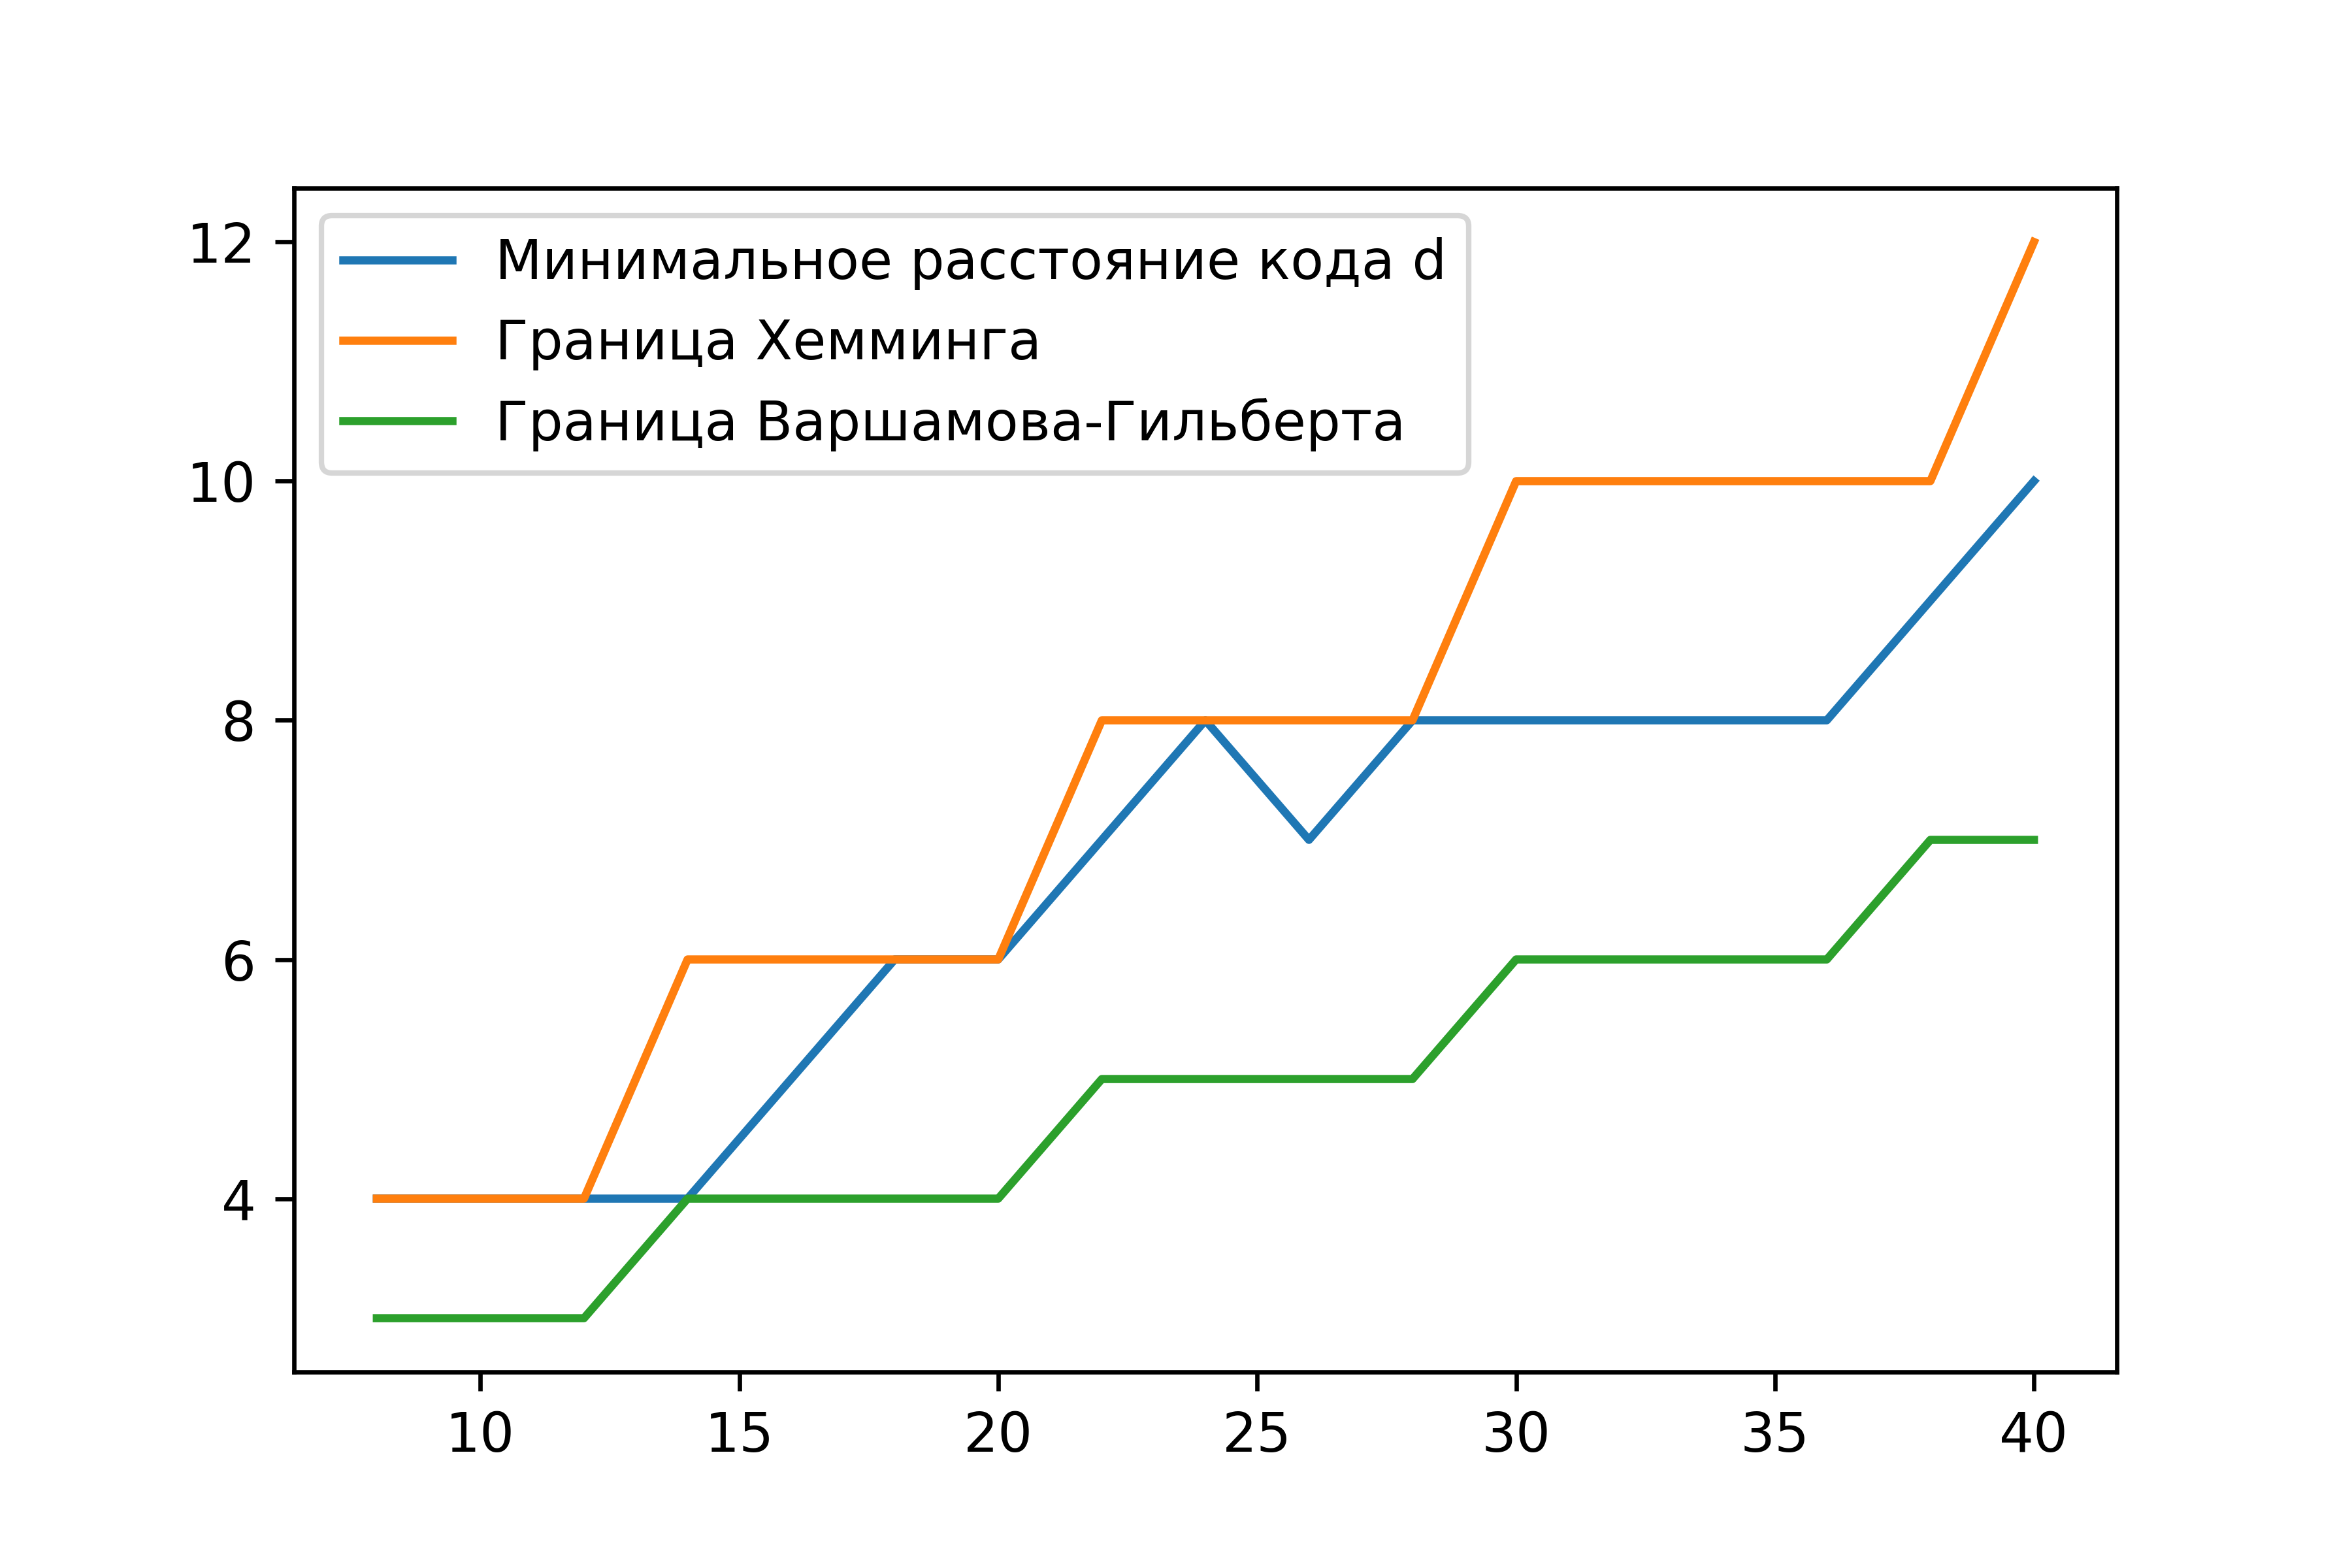
\includegraphics[scale=1]{pic/dist2.png}
\end{document}